\chapter{BOLUM BES BUYUK BASLIK}
\lipsum[1-4]

\newpage
\section{Bölüm 5 alt başlık -1}

\lipsum[6-9]
Bu akış diyagramı detaylı olarak Şekil-\ref{fig:sffffs}'de verilmiştir. 
\lipsum[10-12]

\begin{figure}[htp]%
	\centering
    \begin{tikzpicture}[node distance=2cm]
    
    % \node (start) [startstop] {Başlama};
    \node (in1) [io2] {start};
    \node (pro1) [process2, below of=in1,yshift=-1.0cm] {check};
    \node (dec1) [decision2, below of=pro1, yshift=-3cm] {control?};
    
    \node (pro2) [process2, right of=dec1, xshift=5.0cm] {fit};
    \node (pro3) [process2, below of=dec1, yshift=-2.0cm] {finish};
    % \node (stop) [startstop, below of=out1] {Bitiş};
    
    % \coordinate (point1) at (0cm,-7.3cm);
    % \coordinate (point2) at (4.5cm,-7.3cm);
    % \coordinate (point3) at (4.5cm,-10.5cm); 
    
    % \draw [arrow] (start) -- (in1);
    \draw [arrow] (in1) -- (pro1);
    \draw [arrow] (pro1) -- (dec1);
    \draw [arrow] (pro2) |- (pro1);
    %\draw [arrow] (dec1) -- node {0.232} (pro2);
    \draw [line] (dec1) -- node[pos=0.5, anchor=south] {Yes}(pro2);
    \draw [arrow] (dec1) -- node[anchor=east] {NO} (pro3);
    % \draw [] (dec1) -- (point3);
    % \draw [arrow] (out1) -- (stop);
    
    \end{tikzpicture}
	\caption{flowchart example}%\cite{paper12}.}
	\label{fig:sffffs}%
\end{figure}


\section{Bölüm 5 alt başlık -2}

\lipsum[6-9]
Bu akış diyagramı detaylı olarak Şekil-\ref{fig:sffffs}'de verilmiştir. 
\lipsum[10-11]

\begin{figure}[htp]%
	\centering
    \begin{tikzpicture}[node distance=2cm]
    
    % \node (start) [startstop] {Başlama};
    \node (in1) [io2] {start};
    \node (pro1) [process2, below of=in1,yshift=-1.0cm] {check};
    \node (dec1) [decision2, below of=pro1, yshift=-3cm] {control?};
    
    \node (pro2) [process2, right of=dec1, xshift=5.0cm] {fit};
    \node (pro3) [process2, below of=dec1, yshift=-2.0cm] {finish};
    % \node (stop) [startstop, below of=out1] {Bitiş};
    
    % \coordinate (point1) at (0cm,-7.3cm);
    % \coordinate (point2) at (4.5cm,-7.3cm);
    % \coordinate (point3) at (4.5cm,-10.5cm); 
    
    % \draw [arrow] (start) -- (in1);
    \draw [arrow] (in1) -- (pro1);
    \draw [arrow] (pro1) -- (dec1);
    \draw [arrow] (pro2) |- (pro1);
    %\draw [arrow] (dec1) -- node {0.232} (pro2);
    \draw [line] (dec1) -- node[pos=0.5, anchor=south] {Yes}(pro2);
    \draw [arrow] (dec1) -- node[anchor=east] {NO} (pro3);
    % \draw [] (dec1) -- (point3);
    % \draw [arrow] (out1) -- (stop);
    
    \end{tikzpicture}
	\caption{flowchart example}%\cite{paper12}.}
	\label{fig:7ff7}%
\end{figure}

\newpage
\section{Bölüm 5 alt başlık - 3}
% \lipsum[1-2]
\acrfull{pca}, asdasfasf
\acrshort{pca}'
\lipsum[3]
\parencite{cheng_principal_2022} tarafından yayınlanan Şekil-\ref{fig:apcaaaa} 
\lipsum[15]

\begin{figure}[hbp]
\centering
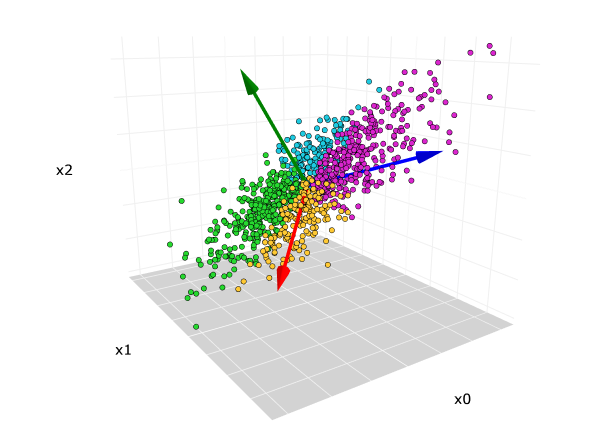
\includegraphics[width=0.69\textwidth]{gorseller/pca_desc.png}
\caption{\acrlong{pca} image}\label{fig:apcaaaa}
\end{figure}
